%% LaTeX-Beamer template for KIT design
%% by Erik Burger, Christian Hammer
%% title picture by Klaus Krogmann
%%
%% version 2.1
%%
%% mostly compatible to KIT corporate design v2.0
%% http://intranet.kit.edu/gestaltungsrichtlinien.php
%%
%% Problems, bugs and comments to
%% burger@kit.edu

\documentclass[18pt]{beamer}

%% SLIDE FORMAT

% use 'beamerthemekit' for standard 4:3 ratio
% for widescreen slides (16:9), use 'beamerthemekitwide'
% for widescreen slide without sidebar use 'beamerthemekitwidenosidebar'

\usepackage{templates/beamerthemekit}
%\usepackage{templates/beamerthemekitwide}
%\usepackage{templates/beamerthemekitwidenosidebar}

% use this to disable the latex beamer navigation symbols
\beamertemplatenavigationsymbolsempty


%% TITLE PICTURE

% if a custom picture is to be used on the title page, copy it into the 'logos'
% directory, in the line below, replace 'mypicture' with the 
% filename (without extension) and uncomment the following line
% (picture proportions: 63 : 20 for standard, 169 : 40 for wide
% *.eps format if you use latex+dvips+ps2pdf, 
% *.jpg/*.png/*.pdf if you use pdflatex)

\titleimage{GoodWillHunting}

%% TITLE LOGO

% for a custom logo on the front page, copy your file into the 'logos'
% directory, insert the filename in the line below and uncomment it

\titlelogo{Graph_K3_3.svg}

% (*.eps format if you use latex+dvips+ps2pdf,
% *.jpg/*.png/*.pdf if you use pdflatex)

%% TikZ INTEGRATION

% use these packages for PCM symbols and UML classes
% \usepackage{templates/tikzkit}
% \usepackage{templates/tikzuml}

% the presentation starts here

\title[IMP]{IMP}
\subtitle{Informatik, Mathematik, Physik}
\author{Malte Vo\ss}

\institute{Abteilung für Didaktik der Mathematik}

\date{29. Januar 2020}

% Bibliography

\usepackage{babelbib}
\bibliographystyle{babplain-lf}
\usepackage{tikz}
\tikzstyle{vertex}=[circle, draw, inner sep=0pt, minimum size=6pt]
\usetikzlibrary[topaths]

\begin{document}

% change the following line to "ngerman" for German style date and logos
\selectlanguage{ngerman}

%title page
\begin{frame}
\titlepage
\end{frame}

%table of contents
\begin{frame}{Gliederung}
\tableofcontents
\end{frame}

\section{IMP}
    \begin{frame}{Profilfach IMP}
        \begin{itemize}[<+->]
            \item IMP ist ein Profilfach
            \item wird in Klassenstufe 8 bis 10 unterrichtet
            \item alternativ zu NWT oder 3. Fremdsprach
            \item vierstündig
            \item Inhalte zu je unterschiedlichen Teilen
        \end{itemize}
    \end{frame}

    \begin{frame}{Lehrplan - inhaltsbezogene Kompetenzen}
        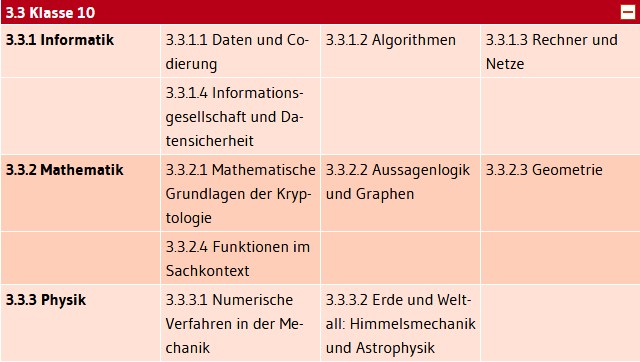
\includegraphics[keepaspectratio, width=\textwidth]{figures/IMP_10}
        \cite{bildungsp}
        \tiny\url{http://www.bildungsplaene-bw.de/,Lde/LS/BP2016BW/ALLG/GYM/IMP}
    \end{frame}

    \begin{frame}{Prozessbezogene Kompetenzen}
    
        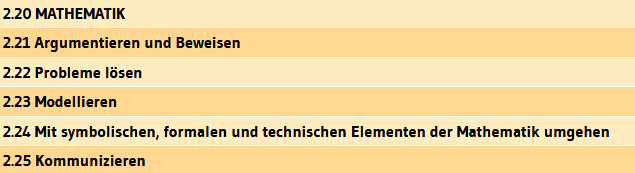
\includegraphics[keepaspectratio, width=0.95\textwidth]{figures/IMP_Prozess.png}
        \cite{bildungsp}
        \pause

    \end{frame}
        


\section{Graphen}
    \begin{frame}{Was sind Graphen?}
        \begin{block}{Formale Definition}
            \glqq Ein gerichteter Graph ist festgelegt durch ein Paar $G = (V, E)$, wobei $E \subset V \times V$ ist\grqq \cite{worsch2016}.
        \end{block}
        \pause
        \begin{block}{etwas handlicher}
            Ein Graph besteht aus Knoten und Kanten, wobei jede Kante zwei Knoten verbindet.
        \end{block}
        \pause
        \begin{block}{etwas mathematischer}
            Ein Graph stellt eine Relation zwischen Objekten dar.
        \end{block}
    \end{frame}

    \begin{frame}[allowframebreaks]{Wozu benutzt man Graphen?}
        \begin{block}{Ein paar Beispiele}
            \begin{itemize}[<+->]
                \item Straßennetz modellieren
                \item Abläufe modellieren
                \item Navigationssysteme
                \item Automaten darstellen
                \item Soziale Netzwerke
                \item Maschinelles Lernen
                \item \dots
            \end{itemize}
        \end{block}
        \begin{figure}[]
            \centering
            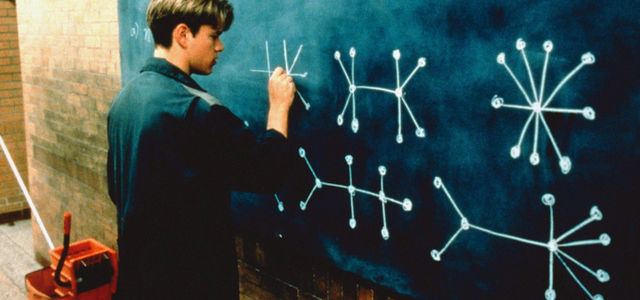
\includegraphics[keepaspectratio,width=\textwidth]{logos/GoodWillHunting.jpg}
            \caption{Good Will Hunting, Gus Van Sant 1997}
        \end{figure}
    \end{frame}

    \begin{frame}{Das Haus vom Nikolaus}
        \begin{align*}
            V & := \{1, \dots, 5\}
            \\
            E & := \bigl\{ \{1,2\}
                         , \{1,5\}
                         , \{2,3\}
                         , \{2,4\}
                         , \{2,5\}
                         , \{3,4\}
                         , \{3,5\}
                         , \{4,5\}
                   \bigr\}
        \end{align*}

        \pause

        \begin{columns}
            \begin{column}{0.5\textwidth}
                \begin{figure}[h]
                    \centering
                    \begin{tikzpicture}
                        \begin{scope}[color=black]
                        \draw[fill] (0,0) circle (2pt);
                        \draw[fill] (1,0) circle (2pt);
                        \draw[fill] (0,1) circle (2pt);
                        \draw[fill] (0.5,1.5) circle (2pt);
                        \draw[fill] (1,1) circle (2pt);
                        \end{scope}
                        \begin{scope}[color=blue]
                        \draw (0.5,1.5) node[above] {$1$};
                        \draw (1,1) node[right] {$2$};
                        \draw (1,0) node[right] {$3$};
                        \draw (0,0) node[left] {$4$};
                        \draw (0,1) node[left] {$5$};
                        \end{scope}
                        \draw[-,rounded corners=0.1cm]
                        (0,0) -- (1,0) -- (0,1) -- (1,1) -- (0,0)
                        -- (0,1) -- (0.5,1.5) -- (1,1) -- (1,0);
                    \end{tikzpicture}
                    \caption{Das Haus vom Nikolaus}
                    \label{fig:hausvomnikolaus}
                \end{figure}
            \end{column}
            \pause
            \begin{column}{0.5\textwidth}
                Besprechung der Hausaufgabe:
                \begin{itemize}
                    \item Grad der Knoten?
                    \item Bedeutung des Grads
                    \item HvN in einem Zug zeichenbar?
                \end{itemize}
            \end{column}
        \end{columns}
    \end{frame}

    \begin{frame}[allowframebreaks]{Königsberger Brückenproblem}
        \begin{figure}
            \centering
            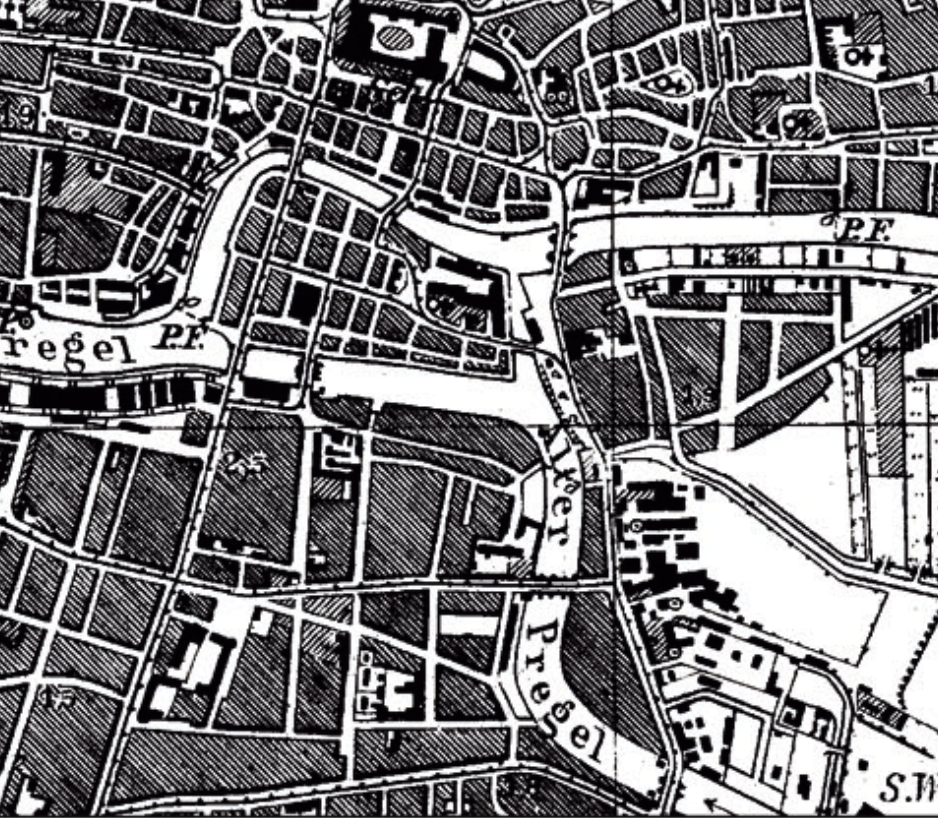
\includegraphics[keepaspectratio,width=180px]{figures/Konigsberg_Brucken_BKG.png}
            \caption{Königsberg 1937 \cite{bkg_kon}}
        \end{figure}

        \framebreak

        \begin{figure}
            \centering
            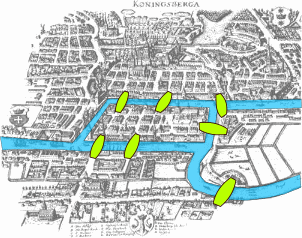
\includegraphics[keepaspectratio,height=130px]{figures/Konigsberg_bridges.png}
            \caption{\tiny \url{wikimedia.org}}
            \glqq Die Einwohner fragten sich, ob es möglich sei, durch die Stadt zu spazieren und dabei alle Brücken genau einmal zu überqueren.\grqq
        \end{figure}
    \end{frame}

    \begin{frame}{}
        \begin{figure}[]
            \centering
            \begin{tikzpicture}
                \node (a) at (0,4) {$a$};
                \node (b) at (0,2) {$b$};
                \node (c) at (0,0) {$c$};
                \node (d) at (4,2) {$d$};
          
                \foreach \from/\to/\pos in {a/b/20,a/b/-20,a/d/0,b/c/20,b/c/-20,b/d/0,c/d/0}
                  \draw[line width=2pt] (\from) to [bend left=\pos] (\to);
            \end{tikzpicture}  
            \caption{Königsberg als Graph}
        \end{figure}  

        \pause
        Begriffe: Eulerweg, -kreis
    \end{frame}

    \begin{frame}{Planare Graphen}
        \begin{columns}
            \begin{column}{0.5\textwidth}
                \begin{figure}[h]
                    \centering
                    \begin{tikzpicture}
                        \begin{scope}[color=black]
                        \draw[fill] (0,0) circle (2pt);
                        \draw[fill] (1,0) circle (2pt);
                        \draw[fill] (0,1) circle (2pt);
                        \draw[fill] (1,1) circle (2pt);
        
                        \draw[fill] (0.35,0.35) circle (2pt);
                        \draw[fill] (1.35,0.35) circle (2pt);
                        \draw[fill] (0.35,1.35) circle (2pt);
                        \draw[fill] (1.35,1.35) circle (2pt);
                        \end{scope}
                        \draw[-] (1.35,0.35) -- (1,0) -- (1,1) -- (0,1) -- (0,0) -- (1,0);
                        \draw[-] (0.35,0.35) -- (1.35,0.35) -- (1.35,1.35) -- (0.35,1.35) -- (0.35,0.35) -- (0,0);
                        \draw[-] (0,1) -- (0.35,1.35);
                        \draw[-] (1,1) -- (1.35,1.35);
                    \end{tikzpicture}
                    \caption{Kantenmodell eines Würfel}
                \end{figure}
            \end{column}
            \pause
            \begin{column}{0.5\textwidth}
                %\draw[fill] 
                \begin{figure}[h]
                    \centering
                    \begin{tikzpicture}
                        \begin{scope}[color=black]
                            \draw[fill] (0,0) circle (2pt);
                            %\draw[fill] (0,1) circle (2pt);
                            %\draw[fill] (0,2) circle (2pt);
                            \draw[fill] (0,3) circle (2pt);
                            %\draw[fill] (1,0) circle (2pt);
                            \draw[fill] (1,1) circle (2pt);
                            \draw[fill] (1,2) circle (2pt);
                            %\draw[fill] (1,3) circle (2pt);
                            %\draw[fill] (2,0) circle (2pt);
                            \draw[fill] (2,1) circle (2pt);
                            \draw[fill] (2,2) circle (2pt);
                            %\draw[fill] (2,3) circle (2pt);
                            \draw[fill] (3,0) circle (2pt);
                            %\draw[fill] (3,1) circle (2pt);
                            %\draw[fill] (3,2) circle (2pt);
                            \draw[fill] (3,3) circle (2pt);
                        \end{scope}
                        \draw[-] (0,0) -- (1,0) -- (2,0) -- (3,0) -- (3,1) -- 
                                    (3,2) -- (3,3) -- (2,3) -- (1,3) -- (0,3)
                                    -- (0,2) -- (0,1) -- (0,0) -- (1,1) -- 
                                    (1,2) -- (2,2) -- (2,1) -- (1,1);
                        \draw[-] (3,0) -- (2,1);
                        \draw[-] (0,3) -- (1,2);
                        \draw[-] (3,3) -- (2,2);
                    \end{tikzpicture}
                    \caption{Der gleiche Graph}
                \end{figure}
            \end{column}
        \end{columns}
        \pause
        \begin{block}{Bemerkung}
            Wenn wir einen Graphen zeichnen können, 
            ohne dass sich Kanten schneiden, 
            nennen wir ihn planar.
        \end{block}
    \end{frame}

    \begin{frame}{Versorger-Verbraucher-Problem}
        \begin{block}{Leitungen}
            Drei Häuser sollen an je drei Versorger angeschlossen werden,
            damit jedes mit Wasser, Strom und Fernwärme versorgt wird.\\
            Die Leitungen dürfen sich nicht kreuzen.
        \end{block}
        \pause
        \begin{itemize}
            \item Betrachte die Versorger und Häuser als Knoten
            \item Die Leitungen stellen Kanten dar
            \item Kanten dürfen sich nicht schneiden
        \end{itemize}
    \end{frame}

% Satz von Kuratowski
    \begin{frame}{Nicht planare Graphen}
        \begin{columns}
            \begin{column}{0.5\textwidth}    
            \begin{figure}
                \centering
                \newcommand\n{5}
                \begin{tikzpicture}
                    \tikzstyle{vertexs}=[draw,fill=black,circle,minimum size=4pt,inner sep=0pt]

                    %the multiplication with floats is not possible. Thus I split the loop in two.
                    \foreach \number in {1,...,\n}{
                        \node[vertexs] (N-\number) at ({\number*(360/\n)}:1.4cm) {};
                    }

                    \foreach \number in {1,...,\n}{
                        \foreach \y in {1,...,\n}{
                            \draw (N-\number) -- (N-\y);
                        }
                    }
                \end{tikzpicture}
                \caption{$K_5$}
            \end{figure}
            \end{column}

            \begin{column}{0.5\textwidth}
                
            
            \begin{figure}[]
                \centering
                \tikzstyle{vertexs}=[draw,fill=black,circle,minimum size=4pt,inner sep=0pt]

                \begin{tikzpicture}
                    \foreach \x in {0,1,2}
                    \foreach \y in {0,1,2}{
                    \node (a)[vertexs] at (2*\y,0) {};
                    \node (b)[vertexs] at (2*\x,2) {};
                        \draw (a) -- (b);
                    }
                \end{tikzpicture}
                \caption{$K_{3,3}$}
            \end{figure}
        \end{column}    
    \end{columns}

    \pause
    \begin{block}{Satz von Kuratowski}
        Graphen, die nicht $K_5$ oder $K_{3,3}$ als
        (topologischen) Minor enthalten sind planar.
    \end{block}
    \end{frame}
% K_{3,3} Versorger-Verbraucher-Problem

    \begin{frame}{Graphen färben}
        \begin{block}{Färbbarkeitsproblem}
            Wie viele Farben brauche ich, damit je zwei benachbarte Knoten
            eines Graphen \emph{nicht} die gleiche Farbe haben?
        \end{block}
        \pause
        \begin{figure}[]
            \centering
            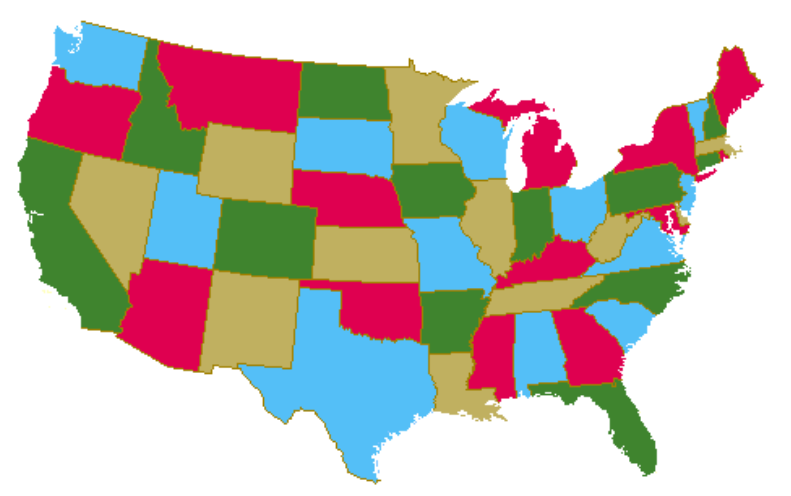
\includegraphics[keepaspectratio, width=.5\textwidth]{figures/usa.png}
            \caption{Bundesstaaten sind Knoten, Nachbarn sind Nachbarn}
        \end{figure}
    \end{frame}

    \begin{frame}{Graphen färben}
        \begin{columns}
            \begin{column}{.5\textwidth}
                \begin{block}{4-Farben-Satz}
                    Planare Graphen sind mit höchstens vier Farben färbbar, um das Färbbarkeitsproblem zu lösen.
                \end{block}
            \end{column}
            \begin{column}{.5\textwidth}
                \begin{figure}[]
                    \centering
                    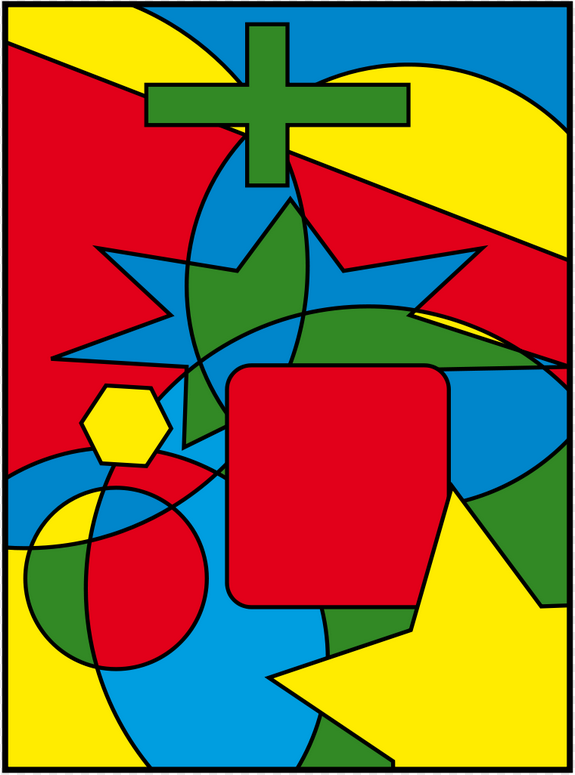
\includegraphics[keepaspectratio, width=.7\textwidth]{figures/4Farben.png}

                    \tiny Von Inductiveload - Based on a this raster image by chas zzz brown on en.wikipedia., 
                    CC BY-SA 3.0, \url{https://commons.wikimedia.org/w/index.php?curid=1680050}
                \end{figure}
            \end{column}
        \end{columns}   
    \end{frame}

    \begin{frame}{Dijkstra-Algorithmus}
        \begin{itemize}[<+->]
            \item berechnet kürzesten Weg in einem Graph von $A$ nach $B$
            \item naive Beschreibung:\\
                Laufe immer die kürzeste bekannte Route vom Startknoten, 
                bis du am Ziel bist.
        \end{itemize}
    \end{frame}

\section{Videos}
    \begin{frame}{Graphen und Euler-Characteristik}
        \begin{block}{Euler-Characteristik}
            \pause
            $\chi = e - k + f$
        \end{block}

        \url{https://www.youtube.com/watch?v=-9OUyo8NFZg}

        \begin{itemize}
            \item Welche neuen Begriffe sind im Video gefallen?
            \item Notiere wichtige Aussagen des Videos.
        \end{itemize}
    \end{frame}

    \appendix
    \beginbackup

    \begin{frame}[allowframebreaks]{Quellen}
    \bibliography{references}
    \end{frame}

    \backupend

    \begin{frame}{Vielen Dank für die Aufmerksamkeit!}
        \begin{figure}[]
            \centering
            
\includegraphics[keepaspectratio, width=0.5\textwidth]{figures/qrcode.png}
            \caption{QR-Code zu \url{http://invote.de/15949}}
        \end{figure}
        
    
    \end{frame}

\end{document}
